% SPDX-FileCopyrightText: 2026 Cyprien PIERRE
% SPDX-License-Identifier: CC-BY-4.0
\documentclass[tikz,border=5pt]{standalone}
\usepackage[T1]{fontenc}
\usepackage{lmodern}
\usetikzlibrary{arrows.meta,positioning}
\begin{document}
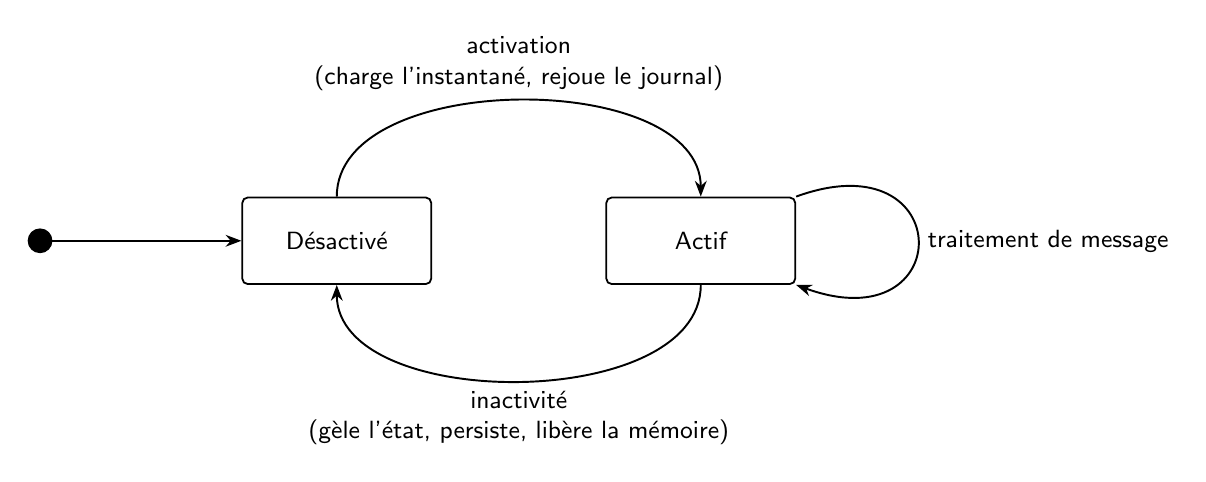
\begin{tikzpicture}[
  font=\sffamily\small,
  initial/.style={circle, fill=black, draw=black, minimum size=3mm, inner sep=0pt},
  state/.style={draw, rounded corners=2pt, minimum height=11mm, minimum width=24mm,
    align=center, line width=.65pt},
  transition/.style={-{Stealth[length=2mm]}, line width=.7pt}
]
\node[initial] (start) {};
\node[state, right=24mm of start] (off) {Désactivé};
\node[state, right=22mm of off] (on) {Actif};
\draw[transition] (start) -- (off);
\draw[transition] (off.north) to[out=90, in=90, looseness=.9]
  node[above, align=center] {activation\\(charge l'instantané, rejoue le journal)} (on.north);
\draw[transition] (on.south) to[out=-90, in=-90, looseness=.9]
  node[below, align=center] {inactivité\\(gèle l'état, persiste, libère la mémoire)} (off.south);
\draw[transition] (on.north east) to[out=20, in=-20, looseness=5]
  node[right] {traitement de message} (on.south east);
\end{tikzpicture}
\end{document}
